\chapter{Introduction}
\label{chap:introduction}

\textit{This chapter introduces the context of the project, together with a brief overview of all the parts that are going to be tackled in the project. It reflects a series of determined objectives that will be addressed during the realization of the project. Besides, the structure of the current document will be presented.
}



\clearpage

\section{Context and motivation}
\label{sec:context}


%%https://www.medigraphic.com/pdfs/revmedcoscen/rmc-2013/rmc133q.pdf
Eating Disorders (EDs) represent, according to the WHO~\cite{baldares2013trastornos}, the most important health problem of humankind, as the number of people affected is increasing, as well as the number of fatalities. They are mental illnesses with a slow recovery period that can become chronic or even lead to death. EDs are real and treatable problems, often occurring alongside other mental illnesses such as depression or substance abuse disorders.

These disorders are part of social and cultural phenomena that transcend the medical field into society. They are influenced by the ideal of beauty that the media disseminate, showing thinness as a symbol of independence and personal and professional success.

%-------------------Definition -------------------

For setting the ground of the main topic tackled in this Master Thesis, the definition of disorders called Eating Disorders is the following: \textit{Eating Disorders are a group of mental disorders that are driven by the development of behaviors aimed at weight control and an altered eating behaviour}~\cite{baldares2013trastornos}. This behavioural disturbance causes functioning problems on a physical and psychosocial level. The main characteristics of these diseases are extreme preoccupation with body and weight and disturbance of eating behaviours. The main representations are Anorexia Nervosa (AN), Bulimia Nervosa (BN) and others unspecified in which Binge Eating is included.


 %-------------------Pandemia de Covid --> efectos secundarios en la salud mental --> problema importante a ser tratado -------------------
% Articulos para esta parte
% 1- https://www.scielosp.org/article/rpmesp/2020.v37n2/327-334/es/
% Conector - https://www.proquest.com/docview/2605236970/fulltextPDF/3291A3310F4C45D6PQ/1?accountid=14712

These psychological problems are context-sensitive as it greatly affects the development of these diseases in more vulnerable patients. An increase in these illnesses has been observed in recent years mainly due to the COVID-19 pandemic. This pandemic started on March 2020 and Spain entered a period of quarantine for several months. Confirmed cases and deaths caused by the virus increased rapidly and as a result of these reasons, the population experienced the development of psychological problems like anxiety, depression and stress, as studies have shown~\cite{ramirez2021repercusiones}.

%The effects of the measures put in place to combat this pandemic have had a notable impact on mental health, increasing the development of inherent illnesses and psychological problems, such as Eating Disorders. 

The risk of suffering from one of these disorders has increased, with patients with no preexisting symptoms being able to develop one of these disorders under certain circumstances. This fact happens because emotional eating is related to biological, psychological and social factors, and the COVID-19 pandemic has been the perfect breeding ground for these types of problems to develop or grow worse~\cite{dos2022emotional}.

%Different studies have shed light on this situation and its importance, as people are having problems with the management of their emotions. It has an impact on population's well-being and in particular on what they eat. It is very important to raise awareness and implement measures to combat the side effects that this pandemic will have in the long term, as the longer it takes, the worse these problems will become~\cite{touyz2020eating}.


 %-------------------Los TCAs estan en alza por x o Y despues de la pandemia, siendo un problema sobre todo en las mujeres jovenes -------------------
% 2- https://onlinelibrary.wiley.com/doi/full/10.1002/eat.23704?casa_token=yKMsm3-JKHYAAAAA%3A_3ZlIvnwecCYorG7JkCITwg2c5b6igm_cyBSPWj7qEvycaCiYDfq0wx3FHOZ1XVi91N3Gi-VCx9JqXU
% Interesantisimo: https://www.behavioralpsycho.com/wp-content/uploads/2021/09/08.Vall_29-2Es.pdf

% Se pueden usar para extender
% NO USADO https://dialnet.unirioja.es/servlet/articulo?codigo=8260225
% NO USADO evolucion EDs en COVID https://aepnya.eu/index.php/revistaaepnya/article/view/850
% NO USADO lo mismo https://www.aepnya.eu/index.php/revistaaepnya/article/view/402

Studies comment the importance of raising awareness and implement measures to combat pandemic side effects~\cite{touyz2020eating}.These studies mentioned above are not based on conjecture, but rather, through an exhaustive and quantitative analysis, such as the studies carried out in various studies like~\cite{j2022impact} or~\cite{vall2021impacto}. 

It has been shown that subjects suffering from an Eating Disorder have experienced deteriorating symptoms, increased isolation and, as a consequence, an increase in hospital admissions as a result of COVID-19. Specifically, it has been found that on average admissions have increased by 48\% compared to pre-pandemic times. In addition, it was found that 36\% of patients' symptoms increased, especially those related to anxiety and depression.

It has also been found that the pandemic has had a major impact on young women between 14 and 35 years of age in the area of mental health problems. These results were shown in demographic studies carried out~\cite{vall2021impacto} which report severe or very severe levels of illness and symptoms. Namely, 30.8\% of the sample analysed suffered from depression, 25.4\% suffered from anxiety and 20.5\% from stress. Significant gender differences were found in terms of eating disorders, and it was found that some life events that these people were suffering that generate stress are related to eating disorders.

In the aforementioned study, the data were processed and a model was generated that related the different terms studied in this Master Thesis, as can be seen in Figure \ref{fig:vall_diagram}. It is possible to appreciate the correlation between them that was observed in the study, being negative between psychological wellbeing and the symptomatologies that occur in mental illnesses. Furthermore, psychological wellbeing is also related to different factors including self-esteem, concern for appearance and self-care, the first two being the ones that have the greatest weight on wellbeing.

\begin{figure}[!htp]
    \centering
    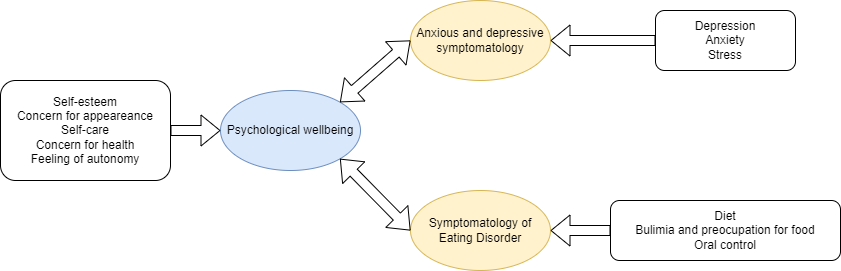
\includegraphics[scale=0.53]{img/introduction/vall_diagram.png}
    \caption{Relational model with the psychological impact of confinement to symptoms~\cite{vall2021impacto}.}
    \label{fig:vall_diagram}
\end{figure}


% ######################## NO SE HA METIDO ########################################
% -------------------Problemas que constan los TCAs --> nivel sanitario y sociologico -------------------
%EAT-26, EAT-40 y SCOFF --> instrumentos para medir frecuencias, chequear para dar numeros en este apartado
% ##################################################################################


% -------------------Social networks and eating disorders (check resources de anteproyecto) -------------------
%Articulo covid + tecnologia + enfermedades mentales: http://www.dspace.uce.edu.ec/handle/25000/25604
% NO USADO -  carta a director anorexia: https://www.scielo.cl/scielo.php?pid=S2452-60532022005000319&script=sci_arttext


This Master Thesis has been developed on the topic of Mental Health and the relationship of this with technology, social networks with the aim of knowing the impact of this.. After an exhaustive literature review, it has been determined that there is a significant association between inappropriate and prolonged use of social networks and the effects of mental health, finding mainly anxious, depressive, stressful and compulsive patterns among others. Therefore, they have determined that social networks can lead to public health problems~\cite{pozo2022impacto}.

From the above, the importance of Eating Disorders after the pandemic has been understood, especially in young women today. Technology and in particular social networks, as a means of communication and expression, play a decisive role in the well-being of current society and particularly, as studied, in the development of these disorders.

Thanks to these, large amounts of information can be extracted and subsequently analysed, processed and used to improve the most critical part of these Eating Disorders, detection. The proposed system in this project will be used to help people to detect and analyse profiles of users potentially suffering from a disorder, in order to speed up the clinical diagnosis process, which is a key factor to take into account when treating a patient with this type of problem.

For implementing this system, we will use Text Classification Techniques for analysing data coming from social networks that will be presented in an engaging user interface easy and quick to use for the user to get a prediction as soon as possible.

%\clearpage

\section{Project goals}
\label{sec:goals}
The goals of this Master Thesis have been designed from the beginning towards developing a social contribution that tackles one problem from the current society: Eating Disorders. With that in mind, the main goal of the present project is to \textbf{develop a system for the analysis and detection of Eating Disorder-related mental health problems in social networks}. The application will integrate artificial intelligence technologies such as Natural Language Processing (NLP) and machine learning to detect these problems working with user data extracted from social media. The purpose of this tool is the \textbf{detection and analysis of user publications referring to Eating Behavior Disorders on social networks}. For this, several sub tasks are required:

\begin{itemize}
    \item Data collection, processing and analysis
    \item Design and implementation of machine learning models able to detect eating disorders from social media
    \item Training and evaluation the proposed models using the obtained datasets
    \item Development of a web application that integrates the proposed models for detecting and analyzing eating disorders
    \item System evaluation in a case study
\end{itemize}

%\clearpage

\section{Structure of this document}

The remaining structure of this document is as follows.

\textbf{\textit{Chapter 2. State of art}}

In this chapter, we will focus on what is already known in different areas that are related to this Master Thesis. In addition. In addition, we will discuss the enabling technologies of
the project.

\textbf{\textit{Chapter 3. Detection}} 

In this chapter we will take a look on the Machine Learning techniques we have applied to get the necessary data to power the project. We will be explanining the data we used, the processing we have performed and which results we got from different models for taking a decision on what is better adjusted to our case.

\textbf{\textit{Chapter 4. Architecture}} 

In this chapter we will break down the design and the patterns followed for implementing the system we want to build in this project.

\textbf{\textit{Chapter 5. Case study}}

Here, the obtained results from the system will be presented for digging into what we have done.

\textbf{\textit{Chapter 6. Conclusions}} 

In this last chapter we will expose the conclusions taken from this Master Thesis and we will complete which are the future lines of work.
